\documentclass[12pt]{article}
\usepackage[T1]{fontenc}
\usepackage[utf8]{inputenc}
\usepackage[spanish]{babel}
\usepackage[letterpaper, portrait, margin=1.3in]{geometry}
\usepackage{coffee3}
\usepackage{graphicx}
\usepackage{fancyhdr}
\usepackage{color}
\usepackage{lipsum}
\usepackage{amsmath}
\usepackage{listings}
\usepackage{mfirstuc}
\usepackage{tikz}
\usepackage{eurosym}
\usepackage{marginnote}

\definecolor{pblue}{rgb}{0.13,0.13,1}
\definecolor{pgreen}{rgb}{0,0.5,0}
\definecolor{pred}{rgb}{0.9,0,0}
\definecolor{pgrey}{rgb}{0.46,0.45,0.48}

\lstset {
    commentstyle=\color{pgreen},
    showstringspaces=false,
    keywordstyle=\color{pblue},
    stringstyle=\color{pred},
    basicstyle=\footnotesize\ttfamily,
    rulecolor=\color{black}
}

\pagestyle{fancy}
\fancyhf{}
\renewcommand{\headrulewidth}{0pt}
\setlength\headheight{25pt}
\fancyhead[L]{\S\ D. Lilue}
\fancyhead[R]{\color{pgrey}\textsc{{\footnotesize \leftmark}}\ $|$ \color{black} \marginnote{\thepage}}
\fancyfoot[R]{\color{pgrey}\footnotesize Universidad Politécnica de Madrid}

\begin{document}

% Title
\begin{center}
    \phantom{x}
    \vfill
    {\Huge \textsc{Maximizar ganancias al asignar vuelos de una aerolínea}}
    \vfill
    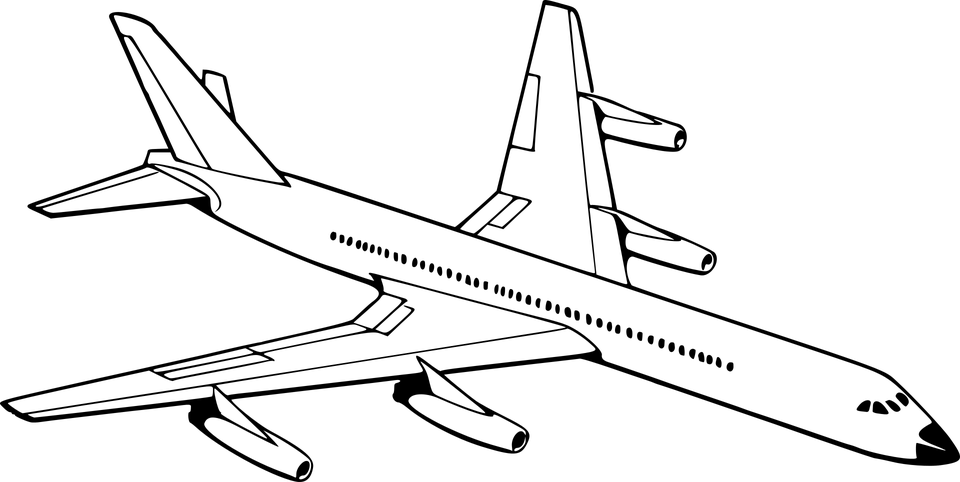
\includegraphics[scale=.23]{./assets/aeroplane-2026921_960_720.png}
    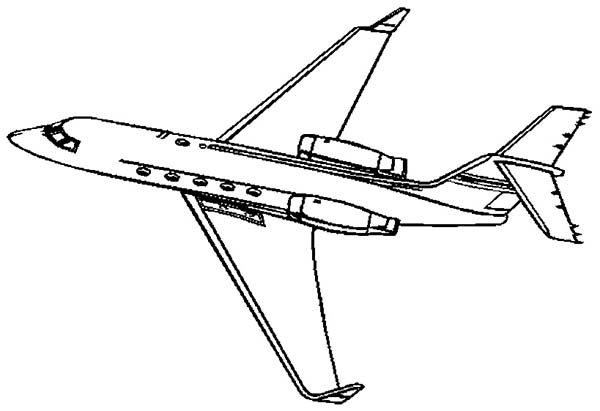
\includegraphics[scale=.37]{./assets/learjet-private-jet-coloring-page.jpg}
    \vfill
    Junio, 2018
    
    \vspace{2em}
    
    {\large David Lilue}
    \vfill
    {\Large Universidad Politécnica de Madrid}

    {\Large Máster en Software y Sistemas}
    \vfill
    %\coffee{1}
\end{center}

\cofeB{0.175}{0.5}{180}

\thispagestyle{empty}

\newpage

\tableofcontents
\listoffigures
\listoftables
\thispagestyle{empty}

\newpage

\section{Introducción}

\lipsum[1-2]

\newpage

\section{Programación lineal}

A través de la programación lineal es posible explorar un espacio de soluciones posibles, con el objetivo de encontrar la óptima. Existen distintos métodos como \emph{Simplex} y el del punto interior, cada una con su propio heurística pero como un mismo fin. Estos técnicas lograr atacar efectivamente problemas que existen en todo tipo de ámbito, con el objetivo de minimizar o maximizar una función. Esta optimización está sujeta un conjunto de restricciones y constantes que permiten reducir el espacio de búsqueda. Con lo cual es posible encontrar solución a problemas adaptados a escenarios de la vida real.

La función objetivo está conformada por variables de decisión, siendo esta un polinomio, la meta es encontrar aquella permutación que logre retornar el menor o mayor resultado; dependiendo de lo que se desee obtener. Por ello, el problema que se presenta en este trabajo se considera dentro del conjunto de los problemas de toma de decisión y en las secciones siguientes se describirá el problema de la programación de vuelos. Encontrando la solución con \texttt{Octave}, un lenguaje de programación \emph{open-source} para resolver problemas de computación numérica; una versión gratuita de \emph{MATLAB}.

\section{Asignación de vuelos}

Este problema tiene como objetivo maximizar las ganancias para una aerolínea, es necesario tomar una decisión en la programación de los vuelos en un día. Dependiendo de una demanda entre un conjunto de ciudades, precio del billete y la opción de usar distintas aeronaves. Además de eso, se especifican las distancia entre las ciudades, la capacidad de cada avión, velocidad, máximo tiempo de utilización y su costo de uso en un periodo de tiempo. A continuación se puede ver gráficamente la distribución de las ciudades y la distancia entre ellas.

\vspace{1em}

\begin{figure}[h]
    \centering
    \begin{tikzpicture}[auto, node distance=3cm, every loop/.style={},
                        thick,main node/.style={circle,draw,font=\sffamily}]
    
      \node[main node] (1) {1};
      \node[main node] (2) [right of=1] {2};
      \node[main node] (3) [above right of=2] {3};
      \node[main node] (4) [below right of=2] {4};
    
      \path[every node/.style={font=\sffamily\small}]
        (1) edge node [above] {260\textsubscript{km}} (2)
        (3) edge node [below right] {375\textsubscript{km}} (2)
        (4) edge node [below left] {310\textsubscript{km}} (2);
    \end{tikzpicture}
    \caption{Grafo de las ciudades}
    \label{fig:cities}
\end{figure}

\paragraph{Demanda}

La demanda de vuelos para cada par de ciudades viene expresada de la siguiente manera. Siendo esta representación útil para resolver el problema en \texttt{Octave} pero sigue teniendo la mismo información que se podría expresar como la figura \ref{fig:cities}.

\begin{table}[h!]
    \centering
    \begin{tabular}{r|r|r|r|r}
        $\lambda_{ij}$%
               &   1  &   2  &   3  &   4\\
            \hline
            \hline
            1  &   0  & 450  &   0  &   0\\
            2  & 600  &   0  & 450  & 760\\
            3  &   0  & 500  &   0  &   0\\
            4  &   0  & 700  &   0  &   0\\
    \end{tabular}
    \caption{Demandas de vuelo}
    \label{tab:demand}
\end{table}

\paragraph{Tasa aérea}

Los costos de los vuelos son iguales independientemente de la dirección en la que se viaje, por lo que el siguiente cuadro es simétrico. A diferencia del anterior (\ref{tab:demand}). Es importante destacar que la unidad de la moneda es indiferente.

\begin{table}[h!]
    \centering
    \begin{tabular}{r|r|r|r|r}
        $f_{ij}$%
               &   1  &   2  &   3  &   4\\
            \hline
            \hline
            1  &   0  & 175  &   0  &   0\\
            2  & 175  &   0  & 230  & 200\\
            3  &   0  & 230  &   0  &   0\\
            4  &   0  & 200  &   0  &   0\\
    \end{tabular}
    \caption{Tasa aérea}
    \label{tab:fare}
\end{table}

\paragraph{Aviones}

En este problema se toman en consideración dos tipos de aeronaves y estas poseen distintas características que se puede ver en el siguiente cuadro. Resaltando 4 aspectos importantes que ayudarán a elaborar las restricciones que ayudarán a conseguir la solución óptima.

\begin{table}[h!]
    \centering
    \begin{tabular}{r|r|r}
        Característica               &    1 &    2\\
        \hline
        \hline
        Capacidad                    &   50 &  100\\
        Velocidad (km/h)             &  400 &  425\\
        Costo de operación (\euro/h) & 1850 & 3800\\
        Uso máximo (h/day)           &   13 &   12\\
    \end{tabular}
    \caption{Tipos de avión}
    \label{tab:planes}
\end{table}

\section{Función objetivo}

Ahora, el primer paso es definir la función que se desea optimizar y decidir si maximizar o minimizar. Para ello, se especifican la variables que definen la solución del problema. En nuestro caso son, número de aviones dado un tipo y el número de vuelos por día desde una ciudad a otro usando cierta aeronave. Formalmente se puede definir de la siguiente manera.

\begin{table}[h!]
    \centering
    \begin{tabular}{r l}
        $P_{k}$   & Número de aviones de tipo $k$\\
        $N_{ijk}$ & Número de vuelos desde $i$ hasta $j$ con el avión $k$\\
         & \\
        $k$ & $= 1,2$\\
        $i,j$ & $= 1,2,3,4$
    \end{tabular}
    \caption{Variables del problema}
    \label{tab:variables}
\end{table}

Como se desea maximizar ganancias, es notorio que el costo del vuelo y la demanda están relacionados, e implican los beneficio de la aerolínea. Usando los cuadros \ref{tab:demand} y \ref{tab:fare}, se puede expresar formalmente la deducción bruta por venta de billetes de la siguiente manera.

\begin{equation}
    \sum_{i,j} \lambda_{ij}.f_{ij}
\end{equation}

Obviamente existe un costo por el uso de las aeronaves y tomando en consideración el número de vuelos de una ciudad a otro usando cierto avión, se puede expresar ese costo con la siguiente ecuación.

\begin{equation}
    \sum_{i,j}\sum_{k} N_{ijk}.C_{ijk}
\end{equation}

Donde $C_{ijk}$ es el costo de volar desde $i$ hasta $j$ usando la aeronave $k$. Los valores de esta matriz de 3 dimensiones se pueden deducir usando la distancia entre dos ciudades, el tiempo que demora cada aeronave y el costo de uso. Dejando el siguiente cuadro como resultado en el caso de la primera aeronave.

\begin{table}[h!]
    \centering
    \begin{tabular}{r|r|r|r|r}
        $C_{ij1}$%
               &   1  &   2  &   3  &   4\\
            \hline
            \hline
              1 &      0 &  2846.2 &       0 &       0\\
              2 & 2846.2 &       0 &  1973.3 &  2387.1\\
              3 &      0 &  1973.3 &       0 &       0\\
              4 &      0 &  2387.1 &       0 &       0\\
    \end{tabular}
    \caption{Costo de volar de i a j con el avión 1}
    \label{tab:cij1}
\end{table}

Y si usamos la segunda aeronave quedaría de la siguiente manera. 

\begin{table}[ht!]
    \centering
    \begin{tabular}{r|r|r|r|r}
        $C_{ij2}$%
               &   1  &   2  &   3  &   4\\
            \hline
            \hline
              1 &      0  & 6211.5  &      0  &      0\\
              2 & 6211.5  &      0  & 4306.7  & 5209.7\\
              3 &      0  & 4306.7  &      0  &      0\\
              4 &      0  & 5209.7  &      0  &      0\\
    \end{tabular}
    \caption{Costo de volar de i a j con el avión 2}
    \label{tab:cij2}
\end{table}

Entonces la función objetivo estaría definida por la ecuaciones descritas anteriormente, con el objetivo de maximizar la ganancia neta.

\begin{equation}
    Max \sum_{i,j} \lambda_{ij}.f_{ij} - \sum_{i,j}\sum_{k} N_{ijk}.C_{ijk}
\end{equation}

O simplemente minimizar los costos de ejecución de la aerolínea, con lo cual quedaría el segundo operando de la resta pero con signo positivo.

\begin{equation}
    Min \sum_{i,j}\sum_{k} N_{ijk}.C_{ijk}
\end{equation}

\section{Restricciones}

Ya que tenemos definida la función objetivo, necesitamos guiar la solución a donde nos interesa, para ello se formalizan las restricciones a las que está sujeto el problema. En primer lugar, nos interesa establecer una relación entre el tiempo de los vuelos y el tiempo que estos están disponibles. Como ya se había mencionado, cada avión tiene un tiempo máximo de uso. En el siguiente apartado se formaliza esta restricción.

\subsection{Máximo uso de las aeronaves}

\begin{equation}
    \sum_{i,j} t_{ijk}.N_{ijk} \leq U_{k}.P_{k},\ \forall k
\end{equation}

Donde $U_k$ es el tiempo de uso máximo de cada avión, este se puede ver en el cuadro \ref{tab:planes}. El tiempo de vuelo entre la ciudad $i$ y $j$ usando la aeronave $k$ se obtiene después de dividir la velocidad de cada avión entre la distancia de la ruta. Los valores obtenidos de esa operación son los siguientes; cada cuadro correspondiente a un tipo de avión.

\newpage

\begin{table}[ht!]
    \centering
    \begin{tabular}{r|r|r|r|r}
        $t_{ij1}$%
               &   1  &   2  &   3  &   4\\
            \hline
            \hline
             1 &      0  & 1.5385  &      0  &      0\\
             2 & 1.5385  &      0  & 1.0667  & 1.2903\\
             3 &      0  & 1.0667  &      0  &      0\\
             4 &      0  & 1.2903  &      0  &      0\\
    \end{tabular}
    \caption{Tiempo de volar de i a j con el avión 1}
    \label{tab:tij1}
\end{table}

\begin{table}[ht!]
    \centering
    \begin{tabular}{r|r|r|r|r}
        $t_{ij2}$%
               &   1  &   2  &   3  &   4\\
            \hline
            \hline
             1 &      0  & 1.6346  &      0  &      0\\
             2 & 1.6346  &      0  & 1.1333  & 1.3710\\
             3 &      0  & 1.1333  &      0  &      0\\
             4 &      0  & 1.3710  &      0  &      0\\
    \end{tabular}
    \caption{Tiempo de volar de i a j con el avión 2}
    \label{tab:tij2}
\end{table}

\subsection{Suplir la demanda}

Una restricción importante, además de maximizar ganancias, es mantener la satisfacción de la clientela. Cubrir la demanda es lo mínimo que se necesita para obtener la mayor ganancia posible, eso para todas las rutas establecidas por la aerolínea. Un factor importante es la capacidad de cada avión, y multiplicando por el número de vuelos, este debe ser mayor o igual a la demanda de una ruta. Formalmente se define esta restricción a continuación.

\begin{equation}
    \sum_{k} n_{k}.N_{ijk} \geq \lambda_{ij},\ \forall (i,j)
\end{equation}

\subsection{Mínimo número de vuelos por ruta}

Para la aerolínea es importante tener un número mínimo de vuelos para cada ruta, este valor es definido de antemano y para nuestro caso se asigno al menos un vuelo por ruta. Es de esperar que se deben sumar los vuelos de ambas aeronaves para definir esta restricción.

\begin{equation}
    \sum_{k} N_{ijk} \geq (N_{ij})_{min},\ \forall (i,j)
\end{equation}

\end{document}